\section{Editor}

Di seguito vengono elencati i casi d'uso per l'editor.

\subsection{Casi d'Uso}


\subsubsection{UC-E0}

    \begin{figure}[H]
      \begin{center}
        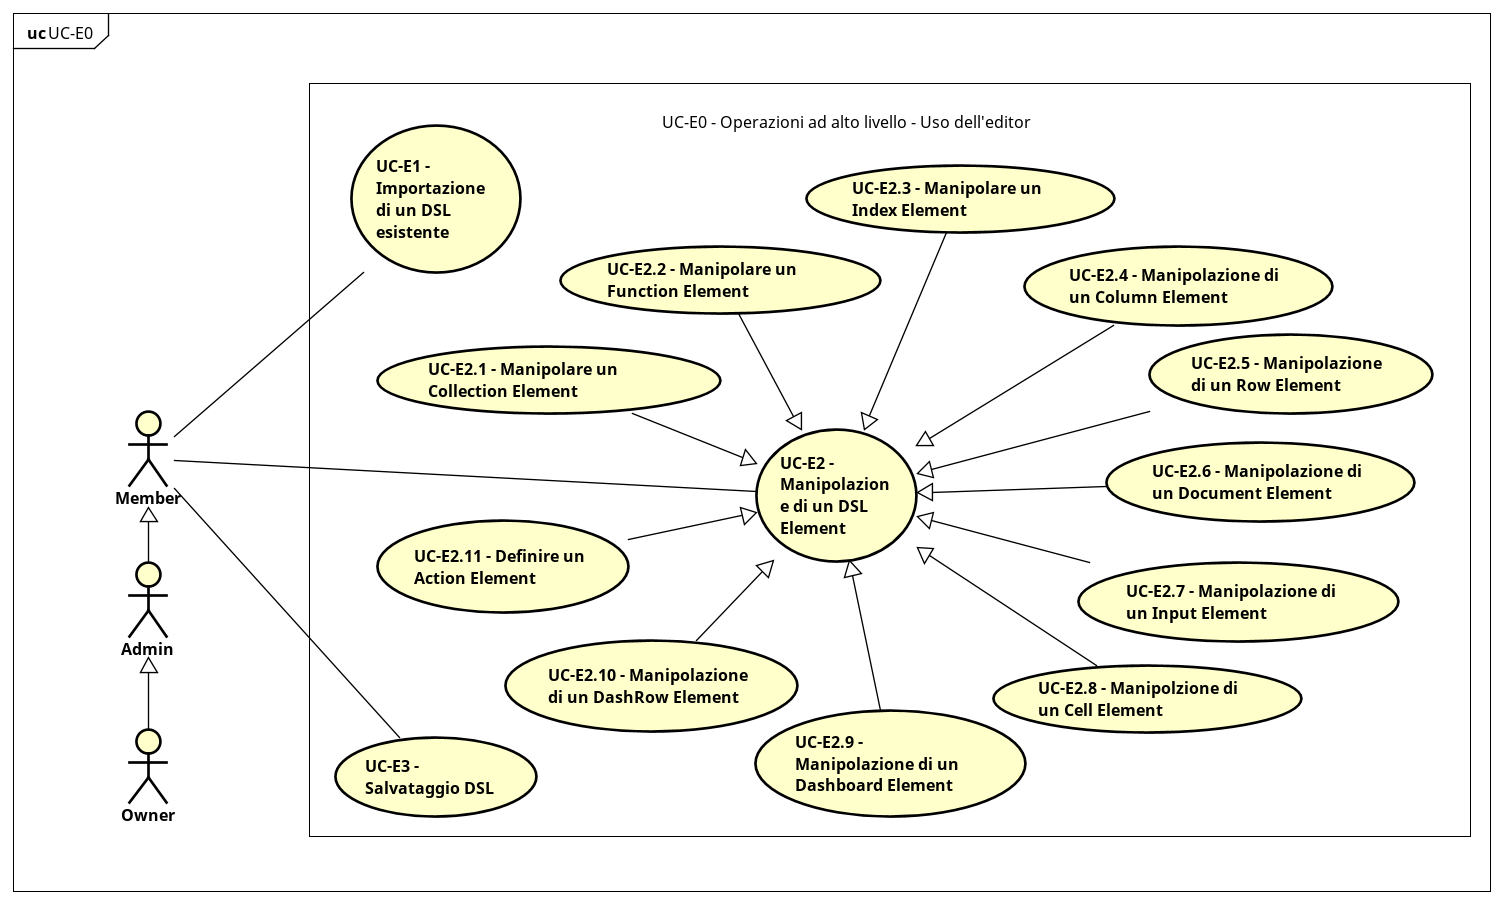
\includegraphics[width=12cm]{res/img/UCEditor/UC-E0.png}
      \caption{UC-E0 - Operazioni ad alto livello - Uso dell'editor}
      \end{center} 
    \end{figure}    
    
    %Tabella 
    \begin{center}
      \bgroup
      \def\arraystretch{1.8}     
      \begin{longtable}{  p{3.5cm} | p{8cm} } 
        
        \hline
        \multicolumn{2}{ | c | }{ \cellcolor[gray]{0.9} \textbf{UC-E0 - Operazioni ad alto livello - Uso dell'editor}} \\ 
        \hline
        
        \textbf{Attori Primari} & Utente Autenticato, Ospite, Membro, Admin, Owner \\ 
        \textbf{Scopo e Descrizione} & L'utente visualizza l'interfaccia dell'Editor tramite cui puo\` svolgere operazioni di importazione di DSL esistenti, manipolazione dei DSL Element e salvataggio del DSL corrente
        \\
        \textbf{Precondizioni}  & L'applicazione dispone l'interfaccia grafica dell'Editor \\ 
        
        \textbf{Postcondizioni} & L'utente ha utilizzato l'editor ed ha eseguito le azioni volute \\ 
        \textbf{Scenario principale} & 1. L'utilizzatore pu\`o importare un DSL esistente. (UC-E1)
2. L'utente pu\`o manipolare un DSL element. (UC-E2)
3. L'utente pu\`o salvare il DSL. (UC-E3)
      \end{longtable}
      \egroup
    \end{center}

    \subsubsection{UC-E1}    
    
    %Tabella 
    \begin{center}
      \bgroup
      \def\arraystretch{1.8}     
      \begin{longtable}{  p{3.5cm} | p{8cm} } 
        
        \hline
        \multicolumn{2}{ | c | }{ \cellcolor[gray]{0.9} \textbf{UC-E1 - Importazione di un DSL esistente}} \\ 
        \hline
        
        \textbf{Attori Primari} & Utente Autenticato, Ospite, Membro, Admin, Owner \\ 
        \textbf{Scopo e Descrizione} & L'utente pu\`o importare un DSL esistente tra quelli personali o quelli della Company. \\ 
        
        \textbf{Precondizioni}  & L'applicazione fornisce la lista di DSL tra cui scegliere quello da importare. \\ 
        
        \textbf{Postcondizioni} & L'applicazione ha caricato con successo il DSL richiesto dall'utente.
      \end{longtable}
      \egroup
    \end{center} 


\subsubsection{UC-E2}

    \begin{figure}[H]
      \begin{center}
        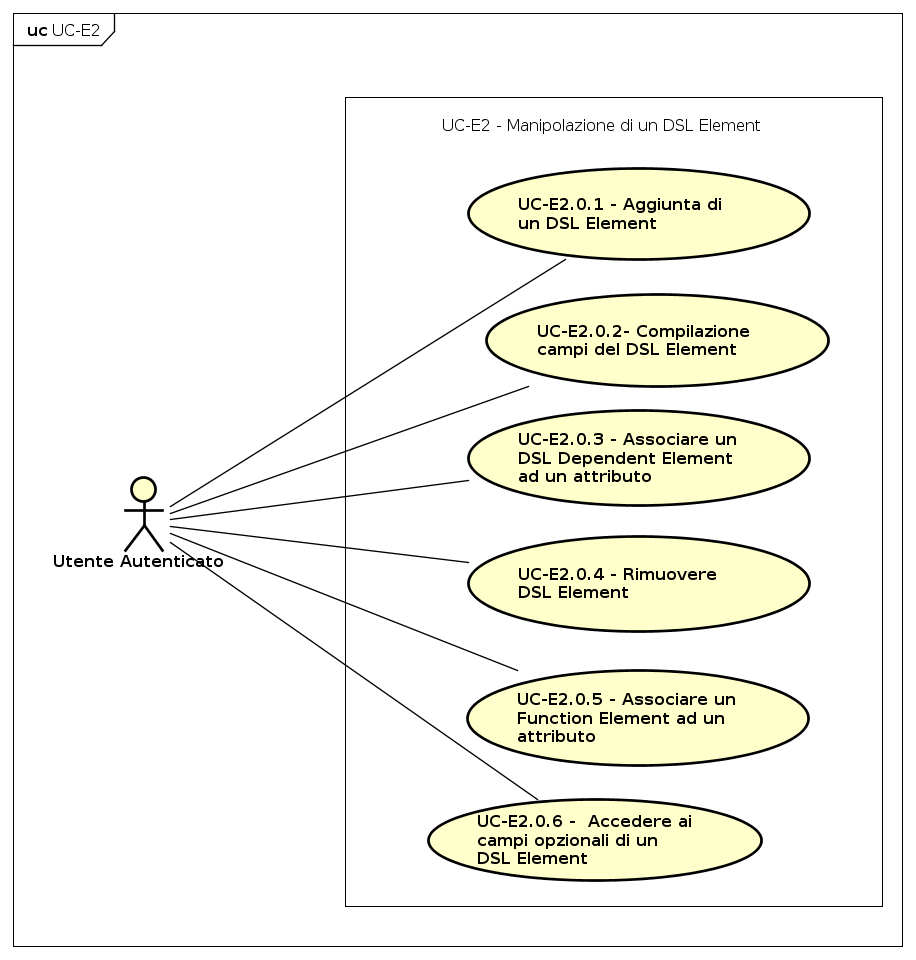
\includegraphics[width=12cm]{res/img/UCEditor/UC-E2.png}
      \caption{UC-E2 - DSL Element}
      \end{center} 
    \end{figure}    
    
    %Tabella 
    \begin{center}
      \bgroup
      \def\arraystretch{1.8}     
      \begin{longtable}{  p{3.5cm} | p{8cm} } 
        
        \hline
        \multicolumn{2}{ | c | }{ \cellcolor[gray]{0.9} \textbf{UC-E2 - Manipolazione di un DSL Element}} \\ 
        \hline
        
        \textbf{Attori Primari} & Utente Autenticato, Ospite, Membro, Admin, Owner \\ 
        \textbf{Scopo e Descrizione} & L'utente pu\`o creare, manipolare o rimuovere un DSL Element all'interno dell'editor. \\ 
        
        \textbf{Precondizioni}  & L'utente visualizza l'editor. \\ 
        
        \textbf{Postcondizioni} & L'utente ha eseguito le sue operazioni sul DSL Element con successo. \\ 
        \textbf{Scenario Principale} & 1. Aggiunta DSL Element (UC-E2.0.1)
2. Compilazione campi (UC-E2.0.2)
3. Collegamento tra un DSL Dependent Element ad un attributo (UC-E2.0.3)
4. Rimuovere DSL Element (UC-E2.0.4)
5. Associare un Function Element (UC-E2.0.5)
6. Accedere ai campi opzionali di un DSL Element (UC-E2.0.6)
      \end{longtable}
      \egroup
    \end{center} 


\subsubsection{UC-E2.0.1}   
    
    %Tabella 
    \begin{center}
      \bgroup
      \def\arraystretch{1.8}     
      \begin{longtable}{  p{3.5cm} | p{8cm} } 
        
        \hline
        \multicolumn{2}{ | c | }{ \cellcolor[gray]{0.9} \textbf{UC-E2.0.1 - Aggiunta di un DSL Element}} \\ 
        \hline
        
        \textbf{Attori Primari} & Utente Autenticato, Ospiete, Membro, Admin, Owner \\ 
        \textbf{Scopo e Descrizione} & L'utente ha la possibiltà di aggiungere un DSL Element e di deciderne il tipo. \\ 
        
        \textbf{Precondizioni}  & L'utente visualizza l'editor. \\ 
        
        \textbf{Postcondizioni} & L'utente ha aggiunto con successo un DSL Element.
      \end{longtable}
      \egroup
    \end{center} 
    
\subsubsection{UC-E2.0.2}

    %Tabella 
    \begin{center}
      \bgroup
      \def\arraystretch{1.8}     
      \begin{longtable}{  p{3.5cm} | p{8cm} } 
        
        \hline
        \multicolumn{2}{ | c | }{ \cellcolor[gray]{0.9} \textbf{UC-E2.0.2 - Compilazione campi del DSL Element}} \\ 
        \hline
        
        \textbf{Attori Primari} & Utente Autenticato, Ospite, Membro, Admin, Owner \\ 
        \textbf{Scopo e Descrizione} & L'utente ha la possibilit\`a di compilare i campi informativi del DSL Element. \\ 
        
        \textbf{Precondizioni}  & L'utente visualizza un DSL Element. \\ 
        
        \textbf{Postcondizioni} & Le informazioni desiderate dall'utente sono stati aggiunte nel DSL Element.
      \end{longtable}
      \egroup
    \end{center}
    
\subsubsection{UC-E2.0.3}

    %Tabella 
    \begin{center}
      \bgroup
      \def\arraystretch{1.8}     
      \begin{longtable}{  p{3.5cm} | p{8cm} } 
        
        \hline
        \multicolumn{2}{ | c | }{ \cellcolor[gray]{0.9} \textbf{UC-E2.0.3 - Associare un DSL Dependent Element ad un attributo}} \\ 
        \hline
        
        \textbf{Attori Primari} & Utente Autenticato, Ospiete, Membro, Admin, Owner \\ 
        \textbf{Scopo e Descrizione} & L'utente ha la possibilit\`a di associare un DSL Dependent Element ad un attributo. \\ 
        
        \textbf{Precondizioni}  & L'utente ha a seleziona un attributo e un DSL Dependent Element da associare. \\ 
        
        \textbf{Postcondizioni} & L'utente ha collegato con successo l'attributo e il DSL Dependent Element.
      \end{longtable}
      \egroup
    \end{center}
\subsubsection{UC-E2.0.4}

    %Tabella 
    \begin{center}
      \bgroup
      \def\arraystretch{1.8}     
      \begin{longtable}{  p{3.5cm} | p{8cm} } 
        
        \hline
        \multicolumn{2}{ | c | }{ \cellcolor[gray]{0.9} \textbf{UC-E2.0.4 - Rimuovere un DSL Element}} \\ 
        \hline
        
        \textbf{Attori Primari} & Utente Autenticato, Ospite, Membro, Admin, Owner \\ 
        \textbf{Scopo e Descrizione} & \`E possibile rimuovere un DSL Element. \\ 
        
        \textbf{Precondizioni}  & L'utente sta visualizzando l'editor e il DSL Element che vuole eliminare \`e presente nell'interfaccia dell'editor. \\ 
        
        \textbf{Postcondizioni} & L'utente ha eliminato con successo il DSL Element selezionato.
      \end{longtable}
      \egroup
    \end{center}
\subsubsection{UC-E2.0.5}

    %Tabella 
    \begin{center}
      \bgroup
      \def\arraystretch{1.8}     
      \begin{longtable}{  p{3.5cm} | p{8cm} } 
        
        \hline
        \multicolumn{2}{ | c | }{ \cellcolor[gray]{0.9} \textbf{UC-E2.0.5 - Associare un Function Element ad un attributo}} \\ 
        \hline
        
        \textbf{Attori Primari} & Utente Autenticato, Ospite, Membro, Admin, Owner \\ 
        \textbf{Scopo e Descrizione} & L'utente ha la possibilit\`a di associare un Function Element ad un attributo selezionabile di un DSL Element. \\ 
        
        \textbf{Precondizioni}  & L'utente visualizza il Function Element e il DSL Element a cui associarlo. \\ 
        
        \textbf{Postcondizioni} & L'utente ha associato con successo la Function Element ad un attributo del DSL Element.
      \end{longtable}
      \egroup
    \end{center}
    
    
\subsubsection{UC-E2.0.6}

    %Tabella 
    \begin{center}
      \bgroup
      \def\arraystretch{1.8}     
      \begin{longtable}{  p{3.5cm} | p{8cm} } 
        
        \hline
        \multicolumn{2}{ | c | }{ \cellcolor[gray]{0.9} \textbf{UC-E2.0.6 - Accedere ai campi opzionali di un DSL Element}} \\ 
        \hline
        
        \textbf{Attori Primari} & Utente Autenticato, Ospite, Membro, Admin, Owner \\ 
        \textbf{Scopo e Descrizione} & L'utente decide di poter aver accesso ai campi opzionali di un DSL Element e a renderli modificabili. \\ 
        
        \textbf{Precondizioni}  & L'utente sta visualizzando uno specifico DSL Element con campi opzionali. \\ 
        
        \textbf{Postcondizioni} & L'utente ha reso modificabili i campi opzionali del DSL Element. Tali campi possono essere modificati come descritto su caso d'uso UC-E2.0.2.
      \end{longtable}
      \egroup
    \end{center}
    
    
    
\subsubsection{UC-E2.1}
 

    \begin{figure}[H]
      \begin{center}
        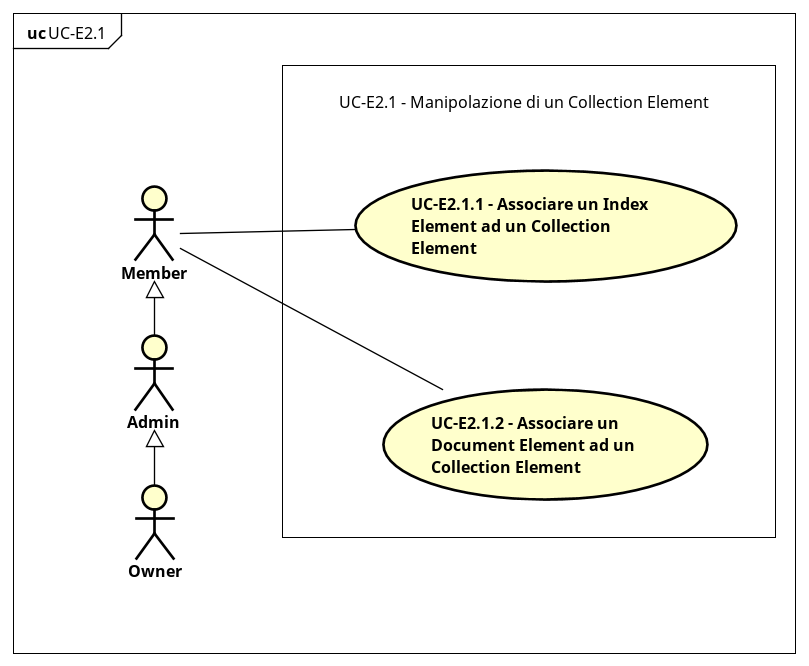
\includegraphics[width=12cm]{res/img/UCEditor/UC-E2.1.png}
      \caption{UC-E2.1 - Collection Element}
      \end{center} 
    \end{figure}

    %Tabella 
    \begin{center}
      \bgroup
      \def\arraystretch{1.8}     
      \begin{longtable}{  p{3.5cm} | p{8cm} } 
        
        \hline
        \multicolumn{2}{ | c | }{ \cellcolor[gray]{0.9} \textbf{UC-E2.1 - Manipolazione di un Collection Element}} \\ 
        \hline
        
        \textbf{Attori Primari} & Utente Autenticato, Ospite, Membro, Admin, Owner \\ 
        \textbf{Scopo e Descrizione} & L'utente pu\`o creare, manipolare o rimuovere un Collection Element all'interno dell'editor. \\ 
        
        \textbf{Precondizioni}  & L'utente sta visualizzando l'editor. \\ 
        
        \textbf{Postcondizioni} & L'utente ha manipolato il Collection Element. \\ 
        \textbf{Scenario principale} & 1. Aggancia un Index Element (UC-E2.1.1)
2. Aggancia un Document Element (UC-E2.1.2) \\
\end{longtable}
      \egroup
    \end{center}
    
    
\subsubsection{UC-E2.1.1}

    %Tabella 
    \begin{center}
      \bgroup
      \def\arraystretch{1.8}     
      \begin{longtable}{  p{3.5cm} | p{8cm} } 
        
        \hline
        \multicolumn{2}{ | c | }{ \cellcolor[gray]{0.9} \textbf{UC-E2.1.1 - Associare un Index Element ad un Collection Element}} \\ 
        \hline
        
        \textbf{Attori Primari} & Utente Autenticato, Ospite, Membro, Admin, Owner \\ 
        \textbf{Scopo e Descrizione} & L'utente ha la possibilit\`a di associare un Index Element all'attributo `index` del Collection Element \\ 
        
        \textbf{Precondizioni}  & Il Collection Element a cui associare l'Index Element \`e visualizzato nell'editor \\ 
        
        \textbf{Postcondizioni} & L'Index Element \`e stato associato ad un Collection Element
      \end{longtable}
      \egroup
    \end{center}
    
    
    
\subsubsection{UC-E2.1.2}

    %Tabella 
    \begin{center}
      \bgroup
      \def\arraystretch{1.8}     
      \begin{longtable}{  p{3.5cm} | p{8cm} } 
        
        \hline
        \multicolumn{2}{ | c | }{ \cellcolor[gray]{0.9} \textbf{UC-E2.1.2 - Associare un Document Element ad un Collection Element}} \\ 
        \hline
        
        \textbf{Attori Primari} & Utente Autenticato, Ospite, Membro, Admin, Owner \\ 
        \textbf{Scopo e Descrizione} & L'utente ha la possibilit\`a di associare un Document Element all'attributo `show` del Collection Element. \\ 
        
        \textbf{Precondizioni}  & Il Collection Element a cui associare il Document Element \`e visualizzato nell'editor.  \\ 
        
        \textbf{Postcondizioni} & Il Document Element \`e stato associato all'attributo `show` del Collection Element desiderato.
      \end{longtable}
      \egroup
    \end{center}
    
    
\subsubsection{UC-E2.2}
    \begin{figure}[H]
      \begin{center}
        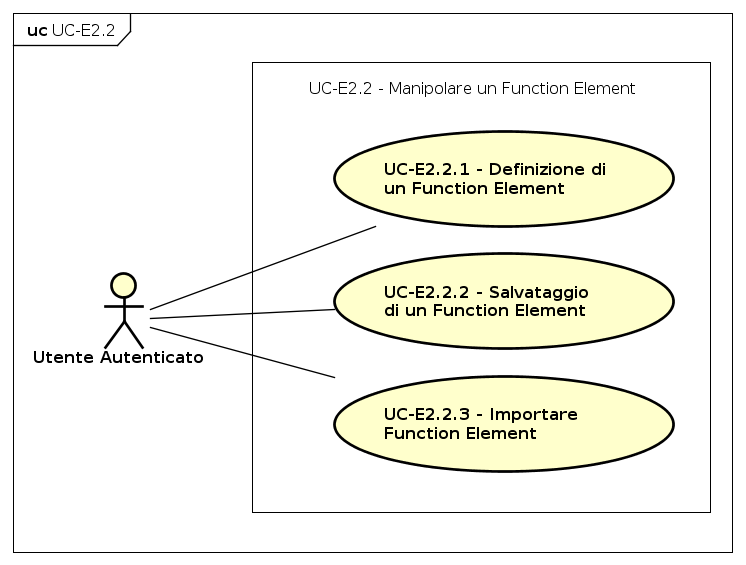
\includegraphics[width=12cm]{res/img/UCEditor/UC-E2.2.png}
      \caption{UC-E2.2 - Manipolare un Function Element}
      \end{center} 
    \end{figure}

    %Tabella 
    \begin{center}
      \bgroup
      \def\arraystretch{1.8}     
      \begin{longtable}{  p{3.5cm} | p{8cm} } 
        
        \hline
        \multicolumn{2}{ | c | }{ \cellcolor[gray]{0.9} \textbf{UC-E2.2 - Manipolare un Function Element}} \\ 
        \hline
        
        \textbf{Attori Primari} & Utente Autenticato, Ospite, Membro, Admin, Owner \\ 
        \textbf{Scopo e Descrizione} & Viene data la possibilit\`a all'utente di creare 
            un Function Element collegabile ad un attributo del DSL Element. \\ 
        
        \textbf{Precondizioni}  & L'editor \`e pronto per l'utilizzo. \\ 
        
        \textbf{Postcondizioni} & L'utente ha creato, modificato o rimosso uno specifico Function Element. \\ 
        \textbf{Scenario principale} & 1. Definire un \textit{function element} (UC-E2.2.1)
2. Salvare Function Element (UC-E2.2.2)
3. Importare Function Element (UC-E2.2.3)  \\
      \end{longtable}
      \egroup
    \end{center}
\subsubsection{UC-E2.2.1}

    %Tabella 
    \begin{center}
      \bgroup
      \def\arraystretch{1.8}     
      \begin{longtable}{  p{3.5cm} | p{8cm} } 
        
        \hline
        \multicolumn{2}{ | c | }{ \cellcolor[gray]{0.9} \textbf{UC-E2.2.1 - Definizione di un Function Element}} \\ 
        \hline
        
        \textbf{Attori Primari} & Utente Autenticato, Ospite, Membro, Admin, Owner \\ 
        \textbf{Scopo e Descrizione} & L'utente ha la possibilit\`a di definire all'interno di un Function Element una funzione nella sintassi del \textit{DSL}. \\ 
        
        \textbf{Precondizioni}  & L'utente sta visualizzando il form di compilazione di un Function Element. \\ 
        
        \textbf{Postcondizioni} & L'utente ha definito con successo una funzione per il Function Element.
      \end{longtable}
      \egroup
    \end{center}
\subsubsection{UC-E2.2.2}

    %Tabella 
    \begin{center}
      \bgroup
      \def\arraystretch{1.8}     
      \begin{longtable}{  p{3.5cm} | p{8cm} } 
        
        \hline
        \multicolumn{2}{ | c | }{ \cellcolor[gray]{0.9} \textbf{UC-E2.2.2 - Salvataggio di un Function Element}} \\ 
        \hline
        
        \textbf{Attori Primari} & Utente Autenticato, Ospite, Membro, Admin, Owner \\ 
        \textbf{Scopo e Descrizione} & L'utente ha la possibilit\`a di salvare il Function Element creato. \\ 
        
        \textbf{Precondizioni}  & L'utente ha inserito un Function Element valido \\ 
        
        \textbf{Postcondizioni} & Il Function Element \`e stata salvato con successo nel sistema.
      \end{longtable}
      \egroup
    \end{center}
    
    
\subsubsection{UC-E2.2.3}

    %Tabella 
    \begin{center}
      \bgroup
      \def\arraystretch{1.8}     
      \begin{longtable}{  p{3.5cm} | p{8cm} } 
        
        \hline
        \multicolumn{2}{ | c | }{ \cellcolor[gray]{0.9} \textbf{UC-E2.2.3 - Importare un Function Element}} \\ 
        \hline
        
        \textbf{Attori Primari} & Utente Autenticato, Ospite, Membro, Admin, Owner \\ 
        \textbf{Scopo e Descrizione} & Il sistema permette di importare un \textit{Function Element} precedentemente definito.\\ 
        
        \textbf{Precondizioni}  & Il sistema fornisce i \textit{Function Element} salvati nel sistema. \\ 
        
        \textbf{Postcondizioni} & L'utente ha caricato il Function Element con successo. \\ 
      \end{longtable}
      \egroup
    \end{center}
    
    
\subsubsection{UC-E2.3}
    \begin{figure}[H]
      \begin{center}
        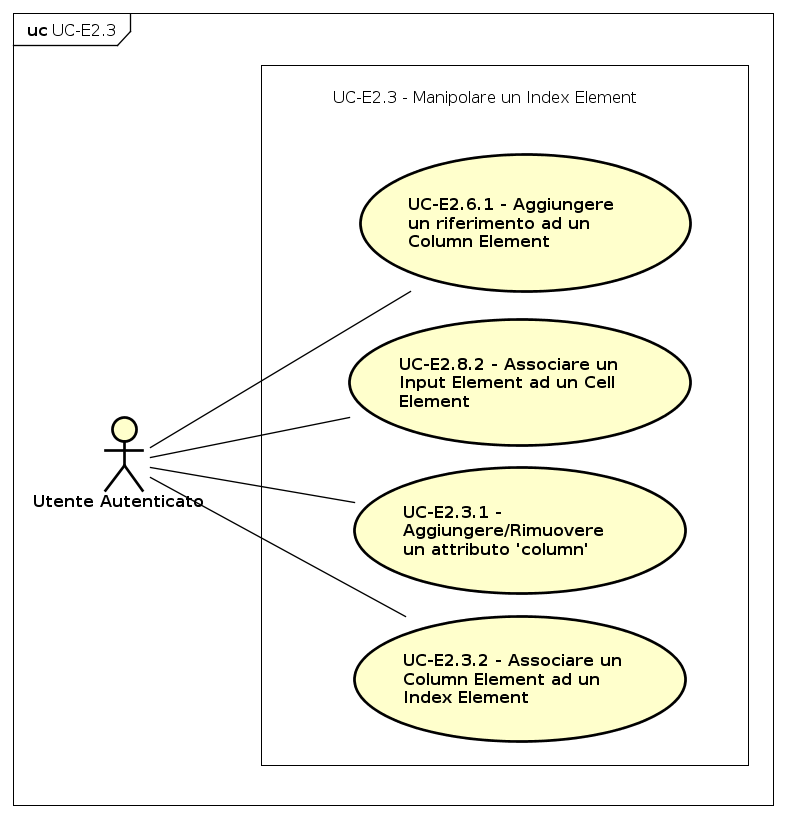
\includegraphics[width=12cm]{res/img/UCEditor/UC-E2.3.png}
      \caption{UC-E2.3 - Index Element}
      \end{center} 
    \end{figure}

    %Tabella 
    \begin{center}
      \bgroup
      \def\arraystretch{1.8}     
      \begin{longtable}{  p{3.5cm} | p{8cm} } 
        
        \hline
        \multicolumn{2}{ | c | }{ \cellcolor[gray]{0.9} \textbf{UC-E2.3 - Manipolare un Index Element}} \\ 
        \hline
        
        \textbf{Attori Primari} & Utente Autenticato, Ospite, Membro, Admin, Owner \\ 
        \textbf{Scopo e Descrizione} & L'utente ha la possibilit\`a di aggiungere, modificare o eliminare un Index Element \\ 
        
        \textbf{Precondizioni}  & L'utente \`e all'interno dell'editor. \\ 
        
        \textbf{Postcondizioni} & \`E stato manipolato l'Index Element secondo le opzioni indicatre dall'utente. \\ 
        \textbf{Scenario Principale} & 1. Aggiungere un riferimento ad un Column Element (UC-E2.6.1)
2. Associare un Input Element (UC-E2.8.2)
3. Aggiungere/Rimuovere un attributo ``column'' (UC-E2.3.1)
4. Associare un Column Element (UC-E2.3.2)
      \end{longtable}
      \egroup
    \end{center}
\subsubsection{UC-E2.3.1}

    %Tabella 
    \begin{center}
      \bgroup
      \def\arraystretch{1.8}     
      \begin{longtable}{  p{3.5cm} | p{8cm} } 
        
        \hline
        \multicolumn{2}{ | c | }{ \cellcolor[gray]{0.9} \textbf{UC-E2.3.1 - Aggiungere/Rimuovere un attributo ``column''}} \\ 
        \hline
        
        \textbf{Attori Primari} & Utente Autenticato, Ospite, Membro, Admin, Owner \\ 
        \textbf{Scopo e Descrizione} & L'utente ha la possibilit\`a di rimuovere o aggiungere dall'Index Element un attributo ``column''. \\ 
        
        \textbf{Precondizioni}  &  L'utente \`e all'interno dell'editor e sta visualizzando un Index Element da modificare. \\ 
        
        \textbf{Postcondizioni} & Il sistema aggiunge un attributo ``column'' all'Index Element modificato.
      \end{longtable}
      \egroup
    \end{center}
\subsubsection{UC-E2.3.2}

    %Tabella 
    \begin{center}
      \bgroup
      \def\arraystretch{1.8}     
      \begin{longtable}{  p{3.5cm} | p{8cm} } 
        
        \hline
        \multicolumn{2}{ | c | }{ \cellcolor[gray]{0.9} \textbf{UC-E2.3.2 - Associare un \textit{Column Element} ad un Index Element}} \\ 
        \hline
        
        \textbf{Attori Primari} & Utente Autenticato, Ospite, Membro, Admin, Owner \\ 
        \textbf{Scopo e Descrizione} & L'utente ha la possibilit\`a di associare un Column Element ad un attributo ``column'' di un Index Element. \\ 
        
        \textbf{Precondizioni}  & L'utente visualizza un Index Element su cui associare il Column Element. \\ 
        
        \textbf{Postcondizioni} & Il sistema associa correttamente il Column Element all Index Element indicato dall'utente.
      \end{longtable}
      \egroup
    \end{center}
    
    
\subsubsection{UC-E2.4}

    %Tabella 
    \begin{center}
      \bgroup
      \def\arraystretch{1.8}     
      \begin{longtable}{  p{3.5cm} | p{8cm} } 
        
        \hline
        \multicolumn{2}{ | c | }{ \cellcolor[gray]{0.9} \textbf{UC-E2.4 - Manipolazione di un Column Element}} \\ 
        \hline
        
        \textbf{Attori Primari} & Utente Autenticato, Ospite, membro, Admin, Owner \\ 
        \textbf{Scopo e Descrizione} & L'utente ha la possibilit\`a di aggiungere, rimuovere o modificare un Column Element \\ 
        
        \textbf{Precondizioni}  & L'editor \`e visualizzato dall'utente. \\ 
        
        \textbf{Postcondizioni} & Il sistema compie le operazioni sul Column Element indicato dall'utente.
      \end{longtable}
      \egroup
    \end{center}
    
\subsubsection{UC-E2.5}

    %Tabella 
    \begin{center}
      \bgroup
      \def\arraystretch{1.8}     
      \begin{longtable}{  p{3.5cm} | p{8cm} } 
        
        \hline
        \multicolumn{2}{ | c | }{ \cellcolor[gray]{0.9} \textbf{UC-E2.5 - Manipolazione di Row Element}} \\ 
        \hline
        
        \textbf{Attori Primari} & Utente Autenticato, Ospite, Membro, Admin, Owner \\ 
        \textbf{Scopo e Descrizione} & L'utente ha la possibilit\`a di aggiungere, rimuovere o modificare un Row Element \\ 
        
        \textbf{Precondizioni}  & L'editor \`e visualizzato dall'utente. \\ 
        
        \textbf{Postcondizioni} & Il sistema compie le operazioni sul Column Element indicato dall'utente.
      \end{longtable}
      \egroup
    \end{center}
\subsubsection{UC-E2.6}
 

    \begin{figure}[H]
      \begin{center}
        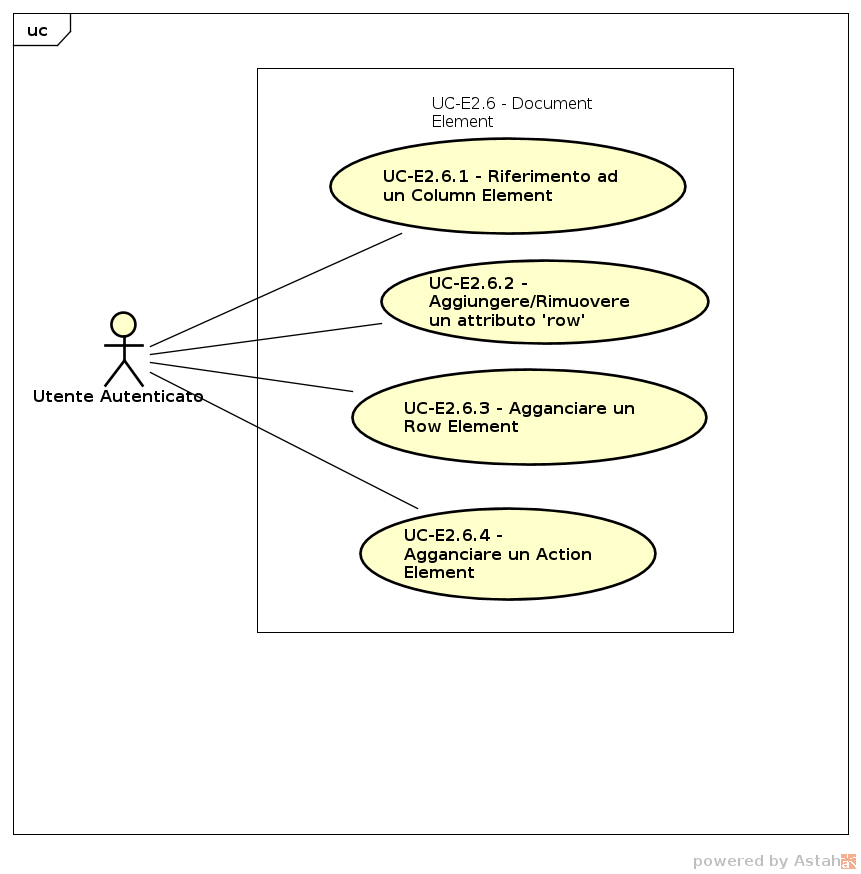
\includegraphics[width=12cm]{res/img/UCEditor/UC-E2.6-DocumentElement}
      \caption{UC-E2.6 - Document Element}
      \end{center} 
    \end{figure}

    %Tabella 
    \begin{center}
      \bgroup
      \def\arraystretch{1.8}     
      \begin{longtable}{  p{3.5cm} | p{8cm} } 
        
        \hline
        \multicolumn{2}{ | c | }{ \cellcolor[gray]{0.9} \textbf{UC-E2.6 - Document Element}} \\ 
        \hline
        
        \textbf{Attori Primari} & Utente Autenticato, Ospite, Membro, Admin, Proprietario \\ 
        \textbf{Scopo e Descrizione} & Rappresenta l'elemento Document del DSL \\ 
        
        \textbf{Precondizioni}  & L'utente visualizza l'editor \\ 
        
        \textbf{Postcondizioni} & Viene generato l'elemento Document nel DSL \\ 
        \textbf{Scenario Principale} & 1. Aggiungere un riferimento ad un Column Element (UC-E2.6.1)
2. Aggiungere/Rimuovere un attributo row (UC-E2.6.2)
3. Agganciare un Row Element (UC-E2.6.3)
4. Agganciare un Action Element (UC-E2.6.4) 
      \end{longtable}
      \egroup
    \end{center}
\subsubsection{UC-E2.6.1}

    %Tabella 
    \begin{center}
      \bgroup
      \def\arraystretch{1.8}     
      \begin{longtable}{  p{3.5cm} | p{8cm} } 
        
        \hline
        \multicolumn{2}{ | c | }{ \cellcolor[gray]{0.9} \textbf{UC-E2.6.1 - Riferimento ad un Column Element}} \\ 
        \hline
        
        \textbf{Attori Primari} & Utente Autenticato, Ospite, Membro, Admin, Proprietario \\ 
        \textbf{Scopo e Descrizione} & Riferirsi ad un elemento colonna precedentemente definito in modo da applicare la populate del DSL \\ 
        
        \textbf{Precondizioni}  & Esista almeno un elemento Document a cui si riferisca \\ 
        
        \textbf{Postcondizioni} & Viene composta la funzione populate
      \end{longtable}
      \egroup
    \end{center}
\subsubsection{UC-E2.6.2}

    %Tabella 
    \begin{center}
      \bgroup
      \def\arraystretch{1.8}     
      \begin{longtable}{  p{3.5cm} | p{8cm} } 
        
        \hline
        \multicolumn{2}{ | c | }{ \cellcolor[gray]{0.9} \textbf{UC-E2.6.2 - Aggiungere/Rimuovere un attributo row}} \\ 
        \hline
        
        \textbf{Attori Primari} & Utente Autenticato, Ospite, Membro, Admin, Proprietario \\ 
        \textbf{Scopo e Descrizione} & Aggiungere o rimuovere una struttura ``row'' all'interno del Document nella struttura DSL \\ 
        
        \textbf{Precondizioni}  & Si deve riferire a un Document esistente \\ 
        
        \textbf{Postcondizioni} & \`E stata manipolata (aggiunta o rimossa) una ``row'' all'interno del DSL Document 
      \end{longtable}
      \egroup
    \end{center}
\subsubsection{UC-E2.6.3}

    %Tabella 
    \begin{center}
      \bgroup
      \def\arraystretch{1.8}     
      \begin{longtable}{  p{3.5cm} | p{8cm} } 
        
        \hline
        \multicolumn{2}{ | c | }{ \cellcolor[gray]{0.9} \textbf{UC-E2.6.3 - Agganciare un Row Element}} \\ 
        \hline
        
        \textbf{Attori Primari} & Utente Autenticato, Ospite, Membro, Admin, Proprietario \\ 
        \textbf{Scopo e Descrizione} & Definire la struttura della ``row'' del DSL  \\ 
        
        \textbf{Precondizioni}  & Sia presente un attributo ``row'' nel Document \\ 
        
        \textbf{Postcondizioni} & Nel DSL vengono trascritti nella struttura ``row'' gli attributi e i rispettivi valori 
      \end{longtable}
      \egroup
    \end{center}
\subsubsection{UC-E2.6.4}

    %Tabella 
    \begin{center}
      \bgroup
      \def\arraystretch{1.8}     
      \begin{longtable}{  p{3.5cm} | p{8cm} } 
        
        \hline
        \multicolumn{2}{ | c | }{ \cellcolor[gray]{0.9} \textbf{UC-E2.6.4 - Agganciare un Action Element}} \\ 
        \hline
        
        \textbf{Attori Primari} & Utente Autenticato, Ospite, Membro, Admin, Proprietario \\ 
        \textbf{Scopo e Descrizione} & Legare il contenuto informativo della ``row'' all'azione definita dalla ``action'' \\ 
        
        \textbf{Precondizioni}  & \`E definita una ``row'' all'interno del DSL \\ 
        
        \textbf{Postcondizioni} & Verr\`a definita la ``action'' nella ``row'' 
      \end{longtable}
      \egroup
    \end{center}
\subsubsection{UC-E2.7}
 

    \begin{figure}[H]
      \begin{center}
        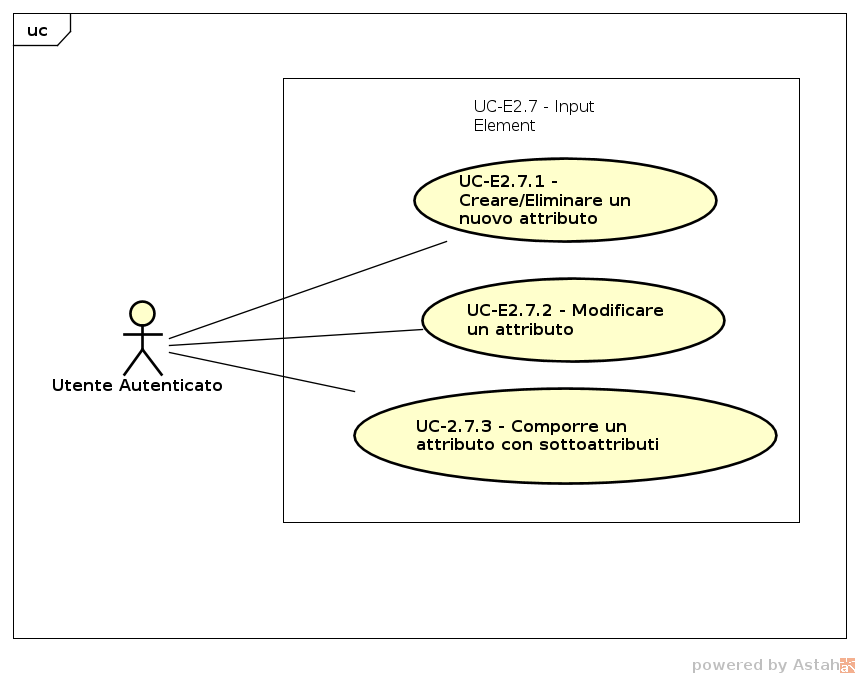
\includegraphics[width=12cm]{res/img/UCEditor/UC-E2.7-InputElement}
      \caption{UC-E2.7 - Input Element}
      \end{center} 
    \end{figure}

    %Tabella 
    \begin{center}
      \bgroup
      \def\arraystretch{1.8}     
      \begin{longtable}{  p{3.5cm} | p{8cm} } 
        
        \hline
        \multicolumn{2}{ | c | }{ \cellcolor[gray]{0.9} \textbf{UC-E2.7 - Input Element}} \\ 
        \hline
        
        \textbf{Attori Primari} & Utente Autenticato, Ospite, Membro, Admin, Proprietario \\ 
        \textbf{Scopo e Descrizione} & Si occupa di rappresentare una dato in un specifico formato \\ 
        
        \textbf{Precondizioni}  & L'utente pu\`o visualizzare l'Editor \\ 
        
        \textbf{Postcondizioni} & Viene composto il dato con i valori inseriti dall'utente \\ 
        \textbf{Scenario Principale} & 1. Creare/Eliminare un nuovo attributo (UC-E2.7.1)
2. Modificare un attributo (UC-E2.7.2)
3. Comporre un attributo con sottoattributi (UC-E2.7.3)
      \end{longtable}
      \egroup
    \end{center}
\subsubsection{UC-E2.7.1}

    %Tabella 
    \begin{center}
      \bgroup
      \def\arraystretch{1.8}     
      \begin{longtable}{  p{3.5cm} | p{8cm} } 
        
        \hline
        \multicolumn{2}{ | c | }{ \cellcolor[gray]{0.9} \textbf{UC-E2.7.1 - Creare/Eliminare un nuovo attributo}} \\ 
        \hline
        
        \textbf{Attori Primari} & Utente Autenticato, Ospite, Membro, Admin, Proprietario \\ 
        \textbf{Scopo e Descrizione} & Essendo il dato componibile da pi\`u attributi, permette di definire una coppia chiave/valore per meglio definire il suo dato \\ 
        
        \textbf{Precondizioni}  & L'utente si deve riferire a un Data Element presente \\ 
        
        \textbf{Postcondizioni} & Si manipola l'attributo selezionato
      \end{longtable}
      \egroup
    \end{center}
\subsubsection{UC-E2.7.2}

    %Tabella 
    \begin{center}
      \bgroup
      \def\arraystretch{1.8}     
      \begin{longtable}{  p{3.5cm} | p{8cm} } 
        
        \hline
        \multicolumn{2}{ | c | }{ \cellcolor[gray]{0.9} \textbf{UC-E2.7.2 - Modificare un attributo}} \\ 
        \hline
        
        \textbf{Attori Primari} & Utente Autenticato, Ospite, Membro, Admin, Proprietario \\ 
        \textbf{Scopo e Descrizione} & Poter rinominare o la chiave o il valore all'interno di un Data Element \\ 
        
        \textbf{Precondizioni}  & Ci sia un attributo a cui riferirsi \\ 
        
        \textbf{Postcondizioni} & Viene modificata o la chiave o il valore dell'attributo selezionato dall'utente
      \end{longtable}
      \egroup
    \end{center}
\subsubsection{UC-E2.7.3}

    %Tabella 
    \begin{center}
      \bgroup
      \def\arraystretch{1.8}     
      \begin{longtable}{  p{3.5cm} | p{8cm} } 
        
        \hline
        \multicolumn{2}{ | c | }{ \cellcolor[gray]{0.9} \textbf{UC-E2.7.3 - Comporre un attributo con sottoattributi}} \\ 
        \hline
        
        \textbf{Attori Primari} & Utente Autenticato, Ospite, Membro, Admin, Proprietario \\ 
        \textbf{Scopo e Descrizione} & Un utente \`e in grado di poter definire strutture complesse per i suoi scopi \\ 
        
        \textbf{Precondizioni}  & Ci sia un Data Element a cui riferirsi \\ 
        
        \textbf{Postcondizioni} & L'attributo del dato \`e a sua volta costituito da altri attributi
      \end{longtable}
      \egroup
    \end{center}
\subsubsection{UC-E2.8}
 

    \begin{figure}[H]
      \begin{center}
        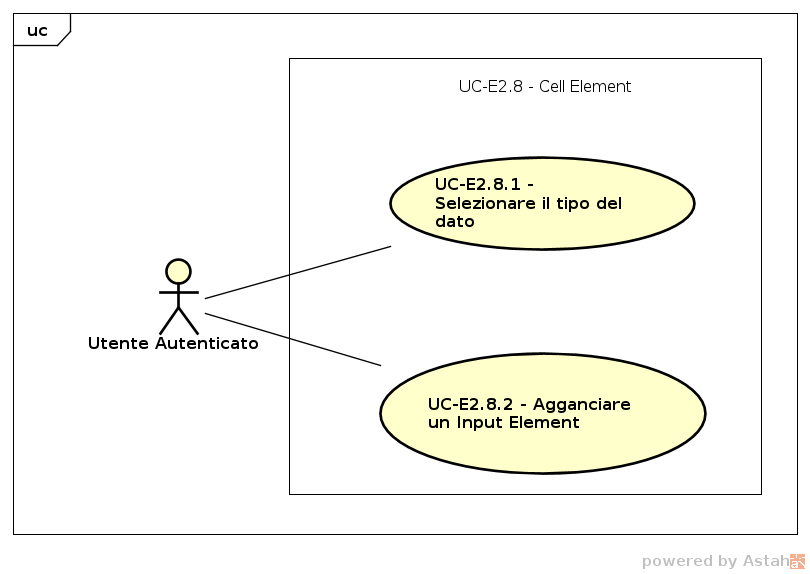
\includegraphics[width=12cm]{res/img/UCEditor/UC-E2.8-CellElement}
      \caption{UC-E2.8 - Cell Element}
      \end{center} 
    \end{figure}

    %Tabella 
    \begin{center}
      \bgroup
      \def\arraystretch{1.8}     
      \begin{longtable}{  p{3.5cm} | p{8cm} } 
        
        \hline
        \multicolumn{2}{ | c | }{ \cellcolor[gray]{0.9} \textbf{UC-E2.8 - Cell Element}} \\ 
        \hline
        
        \textbf{Attori Primari} & Utente Autenticato, Ospite, Membro, Admin, Proprietario \\ 
        \textbf{Scopo e Descrizione} & Rappresentare l'elemento Cell del DSL. \\ 
        
        \textbf{Precondizioni}  & L'utente sta visualizzando l'editor \\ 
        
        \textbf{Postcondizioni} & Viene composta l'elemento Cell nel DSL \\ 
        \textbf{Scenario Principale} &  1. Selezionare il tipo del dato (UC-E2.8.1)
2. Agganciare un Data Element (UC-E2.8.2)
      \end{longtable}
      \egroup
    \end{center}
\subsubsection{UC-E2.8.1}

    %Tabella 
    \begin{center}
      \bgroup
      \def\arraystretch{1.8}     
      \begin{longtable}{  p{3.5cm} | p{8cm} } 
        
        \hline
        \multicolumn{2}{ | c | }{ \cellcolor[gray]{0.9} \textbf{UC-E2.8.1 - Selezionare il tipo del dato}} \\ 
        \hline
        
        \textbf{Attori Primari} & Utente Autenticato, Ospite, Membro, Admin, Proprietario \\ 
        \textbf{Scopo e Descrizione} & Selezionare il tipo di dato da visualizzare, che pu\`o essere:
a. string
b. number
c. link
d. image
e. date \\ 
        
        \textbf{Precondizioni}  & Il tipo di input si deve riferire a un Cell Element \\ 
        
        \textbf{Postcondizioni} & \`E definito nel DSL il tipo di visualizzazione di dato 
      \end{longtable}
      \egroup
    \end{center}
\subsubsection{UC-E2.8.2}

    %Tabella 
    \begin{center}
      \bgroup
      \def\arraystretch{1.8}     
      \begin{longtable}{  p{3.5cm} | p{8cm} } 
        
        \hline
        \multicolumn{2}{ | c | }{ \cellcolor[gray]{0.9} \textbf{UC-E2.8.2 - Agganciare un Input Element}} \\ 
        \hline
        
        \textbf{Attori Primari} & Utente Autenticato, Ospite, Membro, Admin, Proprietario \\ 
        \textbf{Scopo e Descrizione} & Definire quale input il Cell Element rapprensenter\`a \\ 
        
        \textbf{Precondizioni}  & Ci sia un Data Element presente e un Cell Element da collegare \\ 
        
        \textbf{Postcondizioni} & Nel DSL \`e specificato quale valore il Cell Element rappresenta 
      \end{longtable}
      \egroup
    \end{center}
\subsubsection{UC-E2.9}
 

    \begin{figure}[H]
      \begin{center}
        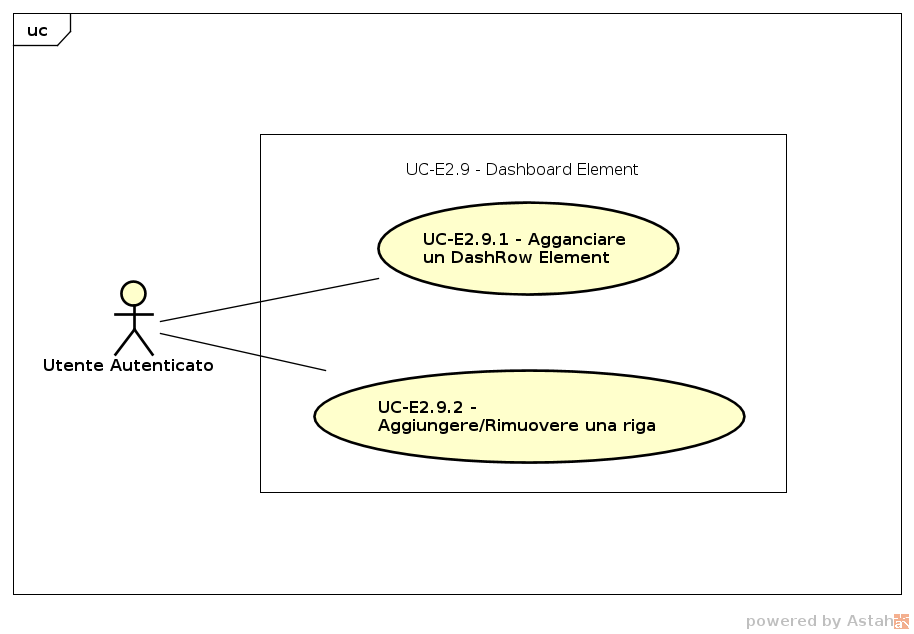
\includegraphics[width=12cm]{res/img/UCEditor/UC-E2.9-DashboardElement}
      \caption{UC-E2.9 - Dashboard Element}
      \end{center} 
    \end{figure}

    %Tabella 
    \begin{center}
      \bgroup
      \def\arraystretch{1.8}     
      \begin{longtable}{  p{3.5cm} | p{8cm} } 
        
        \hline
        \multicolumn{2}{ | c | }{ \cellcolor[gray]{0.9} \textbf{UC-E2.9 - Dashboard Element}} \\ 
        \hline
        
        \textbf{Attori Primari} & Utente Autenticato, Ospite, Membro, Admin, Proprietario \\ 
        \textbf{Scopo e Descrizione} & Rappresentazione di un elemento Dashboard nel DSL \\ 
        
        \textbf{Precondizioni}  & L'utente sta visualizzando l'editor \\ 
        
        \textbf{Postcondizioni} & Viene scritto nel DSL l'elemento Dashboard \\ 
        \textbf{Scenario Principale} & 1. Agganciare un DashRow Element (UC-E2.9.1)
2. Aggiungere/Rimuovere una riga (UC-E2.9.2)
      \end{longtable}
      \egroup
    \end{center}
\subsubsection{UC-E2.9.1}

    %Tabella 
    \begin{center}
      \bgroup
      \def\arraystretch{1.8}     
      \begin{longtable}{  p{3.5cm} | p{8cm} } 
        
        \hline
        \multicolumn{2}{ | c | }{ \cellcolor[gray]{0.9} \textbf{UC-E2.9.1 - Agganciare un DashRow Element}} \\ 
        \hline
        
        \textbf{Attori Primari} & Utente Autenticato, Ospite, Membro, Admin, Proprietario \\ 
        \textbf{Scopo e Descrizione} & Permette di definire la struttura di una Row e di legarla a una Dashboard \\ 
        
        \textbf{Precondizioni}  & Ci sia una Dashboard a cui fare riferimento \\ 
        
        \textbf{Postcondizioni} & Viene inserita nel DSL la configurazione della struttura ``row'' 
      \end{longtable}
      \egroup
    \end{center}
\subsubsection{UC-E2.9.2}

    %Tabella 
    \begin{center}
      \bgroup
      \def\arraystretch{1.8}     
      \begin{longtable}{  p{3.5cm} | p{8cm} } 
        
        \hline
        \multicolumn{2}{ | c | }{ \cellcolor[gray]{0.9} \textbf{UC-E2.9.2 - Aggiungere/Rimuovere una riga}} \\ 
        \hline
        
        \textbf{Attori Primari} & Utente Autenticato, Ospite, Membro, Admin, Proprietario \\ 
        \textbf{Scopo e Descrizione} & Definire una nuova riga all'interno della Dashboard \\ 
        
        \textbf{Precondizioni}  & Ci sia una Dashboard a cui fare riferimento \\ 
        
        \textbf{Postcondizioni} & Viene aggiunto e rimosso un attributo ``row'' 
      \end{longtable}
      \egroup
    \end{center}
\subsubsection{UC-E2.10}
 

    \begin{figure}[H]
      \begin{center}
        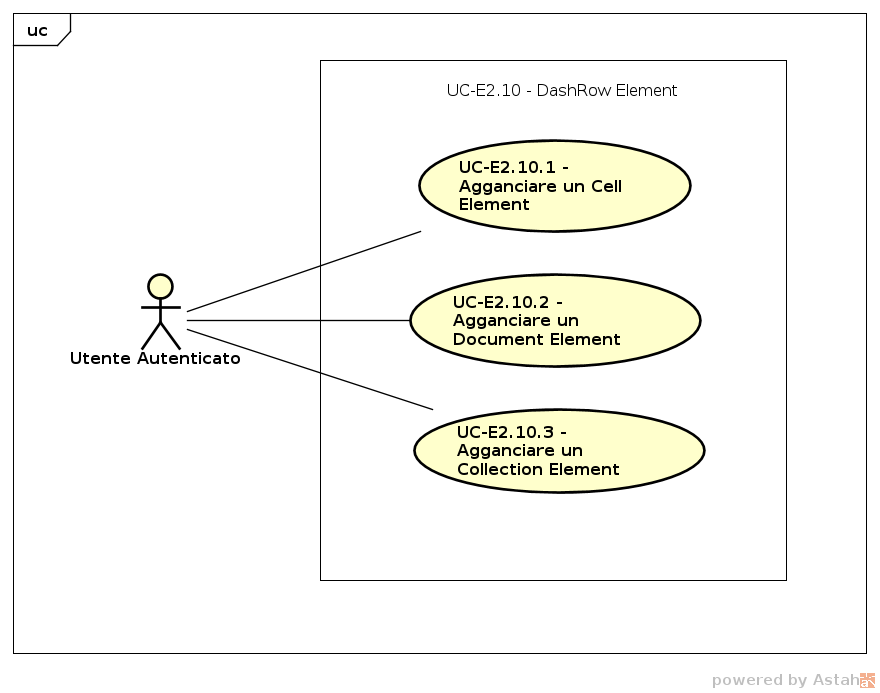
\includegraphics[width=12cm]{res/img/UCEditor/UC-E2.10-DashRowElement}
      \caption{UC-E2.10 - DashRow Element}
      \end{center} 
    \end{figure}

    %Tabella 
    \begin{center}
      \bgroup
      \def\arraystretch{1.8}     
      \begin{longtable}{  p{3.5cm} | p{8cm} } 
        
        \hline
        \multicolumn{2}{ | c | }{ \cellcolor[gray]{0.9} \textbf{UC-E2.10 - DashRow Element}} \\ 
        \hline
        
        \textbf{Attori Primari} & Utente Autenticato, Ospite, Membro, Admin, Proprietario \\ 
        \textbf{Scopo e Descrizione} & Definire la struttura di una ``row'' di una Dashboard in modo che l'utente possa scegliere quale configurazione applicare alla sua Dashboard \\ 
        
        \textbf{Precondizioni}  & Ci sia una Dashboard Element a cui far riferimento \\ 
        
        \textbf{Postcondizioni} & L'utente ha deciso la configurazione della riga della Dashboard \\ 
        \textbf{Scenario Principale} & 1. Agganciare un Cell Element (UC-E2.10.1)
2. Agganciare un Document Element (UC-E2.10.2)
3. Agganciare un Collection Element (UC-E2.10.3)
      \end{longtable}
      \egroup
    \end{center}
\subsubsection{UC-E2.10.1}

    %Tabella 
    \begin{center}
      \bgroup
      \def\arraystretch{1.8}     
      \begin{longtable}{  p{3.5cm} | p{8cm} } 
        
        \hline
        \multicolumn{2}{ | c | }{ \cellcolor[gray]{0.9} \textbf{UC-E2.10.1 - Agganciare un Cell Element}} \\ 
        \hline
        
        \textbf{Attori Primari} & Utente Autenticato, Ospite, Membro, Admin, Proprietario \\ 
        \textbf{Scopo e Descrizione} & Inserire nella riga della Dashboard una colonna rappresentante un Cell del DLS \\ 
        
        \textbf{Precondizioni}  & Ci sia una DashRow Element a cui riferirsi \\ 
        
        \textbf{Postcondizioni} & Nella Row del DSL viene aggiunta una colonna che visualizza un Cell
      \end{longtable}
      \egroup
    \end{center}
\subsubsection{UC-E2.10.2}

    %Tabella 
    \begin{center}
      \bgroup
      \def\arraystretch{1.8}     
      \begin{longtable}{  p{3.5cm} | p{8cm} } 
        
        \hline
        \multicolumn{2}{ | c | }{ \cellcolor[gray]{0.9} \textbf{UC-E2.10.2 - Agganciare un Document Element}} \\ 
        \hline
        
        \textbf{Attori Primari} & Utente Autenticato, Ospite, Membro, Admin, Proprietario \\ 
        \textbf{Scopo e Descrizione} & Inserire nella riga della Dashboard una colonna rappresentante un Document del DLS \\ 
        
        \textbf{Precondizioni}  & Ci sia una DashRow Element a cui riferirsi \\ 
        
        \textbf{Postcondizioni} & Nella Row del DSL viene aggiunta una colonna che visualizza un Document 
      \end{longtable}
      \egroup
    \end{center}
\subsubsection{UC-E2.10.3}

    %Tabella 
    \begin{center}
      \bgroup
      \def\arraystretch{1.8}     
      \begin{longtable}{  p{3.5cm} | p{8cm} } 
        
        \hline
        \multicolumn{2}{ | c | }{ \cellcolor[gray]{0.9} \textbf{UC-E2.10.3 - Agganciare un Collection Element}} \\ 
        \hline
        
        \textbf{Attori Primari} & Utente Autenticato, Ospite, Membro, Admin, Proprietario \\ 
        \textbf{Scopo e Descrizione} & Inserire nella riga della Dashboard una colonna rappresentante un Collection del DLS \\ 
        
        \textbf{Precondizioni}  & Ci sia una DashRow Element a cui riferirsi \\ 
        
        \textbf{Postcondizioni} & Nella Row del DSL viene aggiunta una colonna che visualizza un Collection
      \end{longtable}
      \egroup
    \end{center}
\subsubsection{UC-E2.11}
 

    \begin{figure}[H]
      \begin{center}
        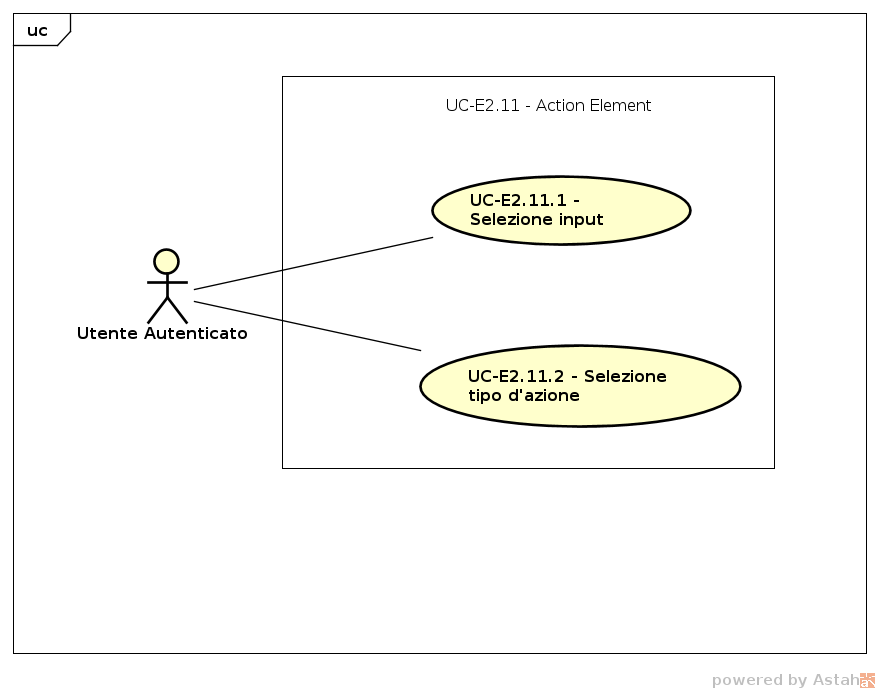
\includegraphics[width=12cm]{res/img/UCEditor/UC-E2.11-ActionElement}
      \caption{UC-E2.11 - Action Element}
      \end{center} 
    \end{figure}

    %Tabella 
    \begin{center}
      \bgroup
      \def\arraystretch{1.8}     
      \begin{longtable}{  p{3.5cm} | p{8cm} } 
        
        \hline
        \multicolumn{2}{ | c | }{ \cellcolor[gray]{0.9} \textbf{UC-E2.11 - Action Element}} \\ 
        \hline
        
        \textbf{Attori Primari} & Utente Autenticato, Ospite, Membro, Admin, Proprietario \\ 
        \textbf{Scopo e Descrizione} & Presentazione dell'Action del DSL nel quale si associa un'input ad una azione definita \\ 
        
        \textbf{Precondizioni}  & Ci dev'essere un documento o una collezione a cui si da riferimento \\ 
        
        \textbf{Postcondizioni} & Si \`e associato a quell'azione o a quel documento l'action desiderato \\ 
        \textbf{Scenario Principale} & 1. Selezione input (UC-E2.11.1)
2. Selezione tipo d'azione (UC-E2.11.2) 
      \end{longtable}
      \egroup
    \end{center}
\subsubsection{UC-E2.11.1}

    %Tabella 
    \begin{center}
      \bgroup
      \def\arraystretch{1.8}     
      \begin{longtable}{  p{3.5cm} | p{8cm} } 
        
        \hline
        \multicolumn{2}{ | c | }{ \cellcolor[gray]{0.9} \textbf{UC-E2.11.1 - Selezione input}} \\ 
        \hline
        
        \textbf{Attori Primari} & Utente Autenticato, Ospite, Membro, Admin, Proprietario \\ 
        \textbf{Scopo e Descrizione} & Selezionare il tipo di Action definite dall'Admin \\ 
        
        \textbf{Precondizioni}  & Ci dev'essere una Collection o un Document a cui fare riferimento \\ 
        
        \textbf{Postcondizioni} & L'Action viene legata all'elemento selezionata come input
      \end{longtable}
      \egroup
    \end{center}
\subsubsection{UC-E2.11.2}

    %Tabella 
    \begin{center}
      \bgroup
      \def\arraystretch{1.8}     
      \begin{longtable}{  p{3.5cm} | p{8cm} } 
        
        \hline
        \multicolumn{2}{ | c | }{ \cellcolor[gray]{0.9} \textbf{UC-E2.11.2 - Selezione tipo d'azione}} \\ 
        \hline
        
        \textbf{Attori Primari} & Utente Autenticato, Ospite, Membro, Admin, Proprietario \\ 
        \textbf{Scopo e Descrizione} & L'utente pu\`o definire l'azione legata all'Action \\ 
        
        \textbf{Precondizioni}  & C'\`e un'Action a cui fa riferimento \\ 
        
        \textbf{Postcondizioni} & L'utente ha definito quali azioni intraprendere eseguendo quell'Action 
      \end{longtable}
      \egroup
    \end{center}
\subsubsection{UC-E3}
 

    \begin{figure}[H]
      \begin{center}
        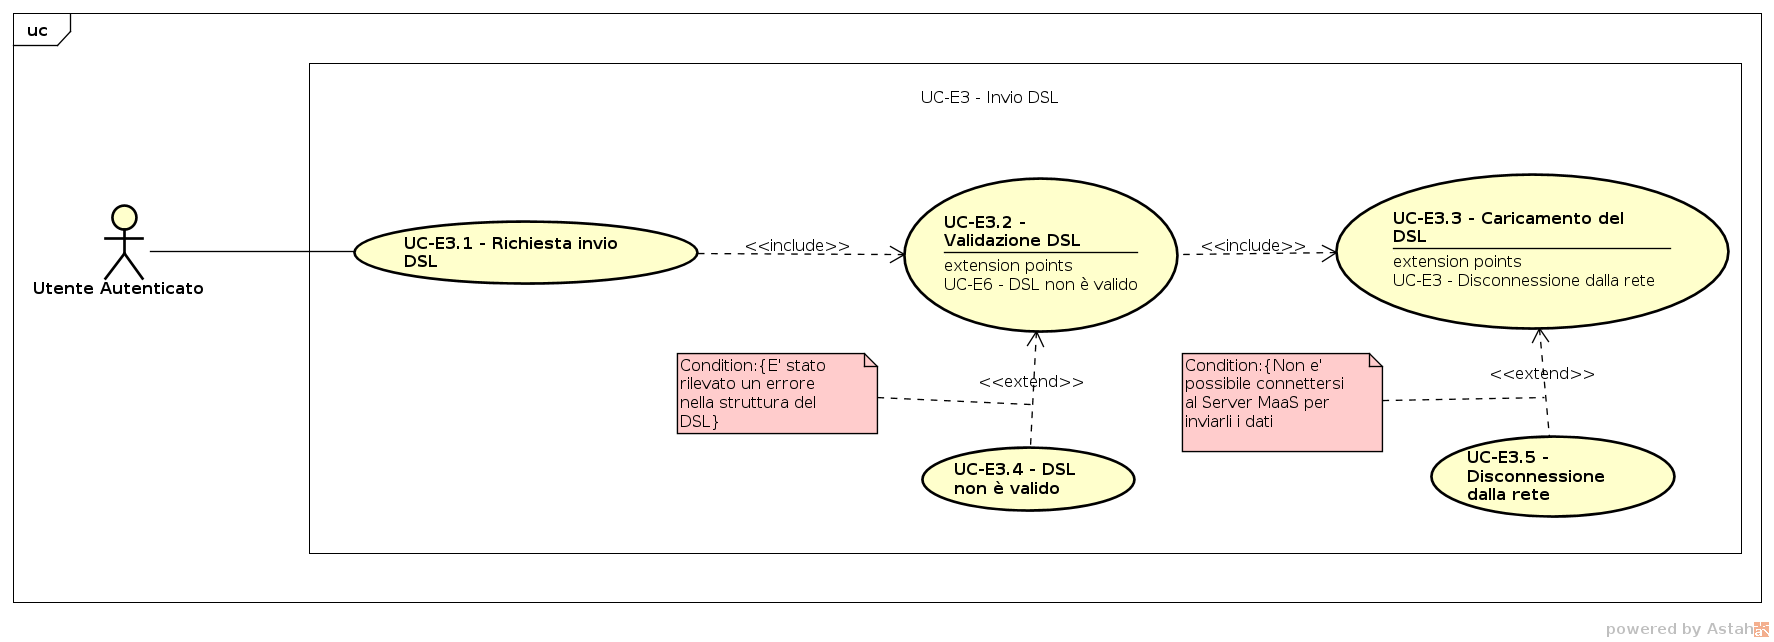
\includegraphics[width=12cm]{res/img/UCEditor/UC-E3}
      \caption{UC-E3 - Invio DSL}
      \end{center} 
    \end{figure}

    %Tabella 
    \begin{center}
      \bgroup
      \def\arraystretch{1.8}     
      \begin{longtable}{  p{3.5cm} | p{8cm} } 
        
        \hline
        \multicolumn{2}{ | c | }{ \cellcolor[gray]{0.9} \textbf{UC-E3 - Invio DSL}} \\ 
        \hline
        
        \textbf{Attori Primari} & Utente Autenticato, Ospite, Membro, Admin, Proprietario \\ 
        \textbf{Scopo e Descrizione} & Inviare la DSL al server per salvarla ed eseguirla \\ 
        
        \textbf{Precondizioni}  & L'utente visualizza l'editor \\ 
        
        \textbf{Postcondizioni} & Il DSL \`e stato caricato con successo sul MaaS ed eseguito \\ 
        \textbf{Scenario Principale} & 1. Richiesta invio DSL (UC-E3.1) 
      \end{longtable}
      \egroup
    \end{center}
\subsubsection{UC-E3.1}

    %Tabella 
    \begin{center}
      \bgroup
      \def\arraystretch{1.8}     
      \begin{longtable}{  p{3.5cm} | p{8cm} } 
        
        \hline
        \multicolumn{2}{ | c | }{ \cellcolor[gray]{0.9} \textbf{UC-E3.1 - Richiesta invio DSL}} \\ 
        \hline
        
        \textbf{Attori Primari} & Utente Autenticato, Ospite, Membro, Admin, Proprietario \\ 
        \textbf{Scopo e Descrizione} & L'utente chiede al programma dell'editor di eseguire tutte le operazioni necessarie affinch\`e ci sia l'invio del DSL al server e la sua esecuzione \\ 
        
        \textbf{Precondizioni}  & L'utente visualizza l'Editor \\ 
        
        \textbf{Postcondizioni} & Si sono avviate tutte le procedure dell'editor per eseguire i passi necessari per l'invio del DSL
      \end{longtable}
      \egroup
    \end{center}
\subsubsection{UC-E3.2}

    %Tabella 
    \begin{center}
      \bgroup
      \def\arraystretch{1.8}     
      \begin{longtable}{  p{3.5cm} | p{8cm} } 
        
        \hline
        \multicolumn{2}{ | c | }{ \cellcolor[gray]{0.9} \textbf{UC-E3.2 - Validazione DSL}} \\ 
        \hline
        
        \textbf{Attori Primari} &  \\ 
        \textbf{Scopo e Descrizione} & Al DSL creato vengano eseguiti tutti i controlli affinch\`e il parser possa interpretarli in maniera corretta \\ 
        
        \textbf{Precondizioni}  & L'utente ha fatto richiesta di invio del DSL \\ 
        
        \textbf{Postcondizioni} & Il DSL \`e stato correttamente validato e la sua correttezza \`e stata garantita \\ 
        \textbf{Estensioni} & 1. DSL non \`e valido (UC-E3.4)
      \end{longtable}
      \egroup
    \end{center}
\subsubsection{UC-E3.3}

    %Tabella 
    \begin{center}
      \bgroup
      \def\arraystretch{1.8}     
      \begin{longtable}{  p{3.5cm} | p{8cm} } 
        
        \hline
        \multicolumn{2}{ | c | }{ \cellcolor[gray]{0.9} \textbf{UC-E3.3 - Caricamento del DSL}} \\ 
        \hline
        
        \textbf{Attori Primari} &  \\ 
        \textbf{Scopo e Descrizione} & Inviare al server il DSL valido affinch\`e possa essere eseguito \\ 
        
        \textbf{Precondizioni}  & Il DSL deve essere valido \\ 
        
        \textbf{Postcondizioni} & Il DSL \`e stato correttamente caricato nel server MaaS \\ 
        \textbf{Estensioni} & 1. Disconnessione dalla rete (UC-E3.5) \\
      \end{longtable}
      \egroup
    \end{center}
\subsubsection{UC-E3.4}

    %Tabella 
    \begin{center}
      \bgroup
      \def\arraystretch{1.8}     
      \begin{longtable}{  p{3.5cm} | p{8cm} } 
        
        \hline
        \multicolumn{2}{ | c | }{ \cellcolor[gray]{0.9} \textbf{UC-E3.4 - DSL non `e valido}} \\ 
        \hline
        
        \textbf{Attori Primari} &  \\ 
        \textbf{Scopo e Descrizione} & Avvisare l'utente dove si trovano gli errori nel DSL definito \\ 
        
        \textbf{Precondizioni}  & Il DSL non \`e corretto \\ 
        
        \textbf{Postcondizioni} & L'utente \`e stato avvisato tramite un messaggio dove sono gli errori
      \end{longtable}
      \egroup
    \end{center}
\subsubsection{UC-E3.5}

    %Tabella 
    \begin{center}
      \bgroup
      \def\arraystretch{1.8}     
      \begin{longtable}{  p{3.5cm} | p{8cm} } 
        
        \hline
        \multicolumn{2}{ | c | }{ \cellcolor[gray]{0.9} \textbf{UC-E3.5 - Disconnessione dalla rete}} \\ 
        \hline
        
        \textbf{Attori Primari} &  \\ 
        \textbf{Scopo e Descrizione} & Avvisare l'utente dell'impossibilit\`a di effettuare il caricamento del DSL sul server \\ 
        
        \textbf{Precondizioni}  & Non \`e pi\`u possibile comunicare con il server MaaS \\ 
        
        \textbf{Postcondizioni} & L'utente \`e stato avvisato con un messaggio di errore dell'impossibilit\`a di caricare il DSL sul server MaaS 
      \end{longtable}
      \egroup
    \end{center}
